\documentclass[a4paper, 12pt]{report}
\usepackage{cmap}
\usepackage{amssymb}
\usepackage{amsmath}
\usepackage{graphicx}
\usepackage{amsthm}
\usepackage{upgreek}
\usepackage{setspace}
\usepackage[T2A]{fontenc}
\usepackage[utf8]{inputenc}
\usepackage[normalem]{ulem}
\usepackage{mathtext} % русские буквы в формулах
\usepackage[left=2cm,right=2cm, top=2cm,bottom=2cm,bindingoffset=0cm]{geometry}
\usepackage[english,russian]{babel}
\usepackage[unicode]{hyperref}
\newenvironment{Proof} % имя окружения
{\par\noindent{$\blacklozenge$}} % команды для \begin
{\hfill$\scriptstyle\boxtimes$}
\newcommand{\grad}{\operatorname{grad}}
\newcommand{\Rm}{\mathbb{R}}
\newcommand{\Cm}{\mathbb{C}}
\newcommand{\Z}{\mathbb{Z}}
\newcommand{\I}{\mathbb{I}}
\newcommand{\N}{\mathbb{N}}
\newcommand{\rank}{\operatorname{rank}}
\newcommand{\Ra}{\Rightarrow}
\newcommand{\ra}{\rightarrow}
\newcommand{\FI}{\Phi}
\newcommand{\Sp}{\text{Sp}}
\renewcommand{\leq}{\leqslant}
\renewcommand{\geq}{\geqslant}
\renewcommand{\alpha}{\upalpha}
\renewcommand{\beta}{\upbeta}
\renewcommand{\gamma}{\upgamma}
\renewcommand{\delta}{\updelta}
\renewcommand{\varphi}{\upvarphi}
\renewcommand{\tau}{\uptau}
\renewcommand{\lambda}{\uplambda}
\renewcommand{\psi}{\uppsi}
\renewcommand{\mu}{\upmu}
\renewcommand{\omega}{\upomega}
\renewcommand{\d}{\partial}
\renewcommand{\xi}{\upxi}
\renewcommand{\epsilon}{\upvarepsilon}
\newcommand{\intx}{\int\limits_{x_0}^x}
\newcommand\Norm[1]{\left\| #1 \right\|}
\newcommand{\Ln}{L_n = D^n + a_{n-1}D^{n-1} + \ldots + a_1D + a_0D^0}
\newcommand{\KFunc}{\int\limits_{t_0}^{t}\varphi_{n-1}(t-\uptau)f(\uptau)d\uptau}
\newcommand{\sumk}{\sum\limits_{k=0}^\infty}
\newcommand{\sumi}{\sum\limits_{i=0}^\infty}
\newtheorem*{theorem}{Теорема}
\newtheorem*{cor}{Следствие}
\newtheorem*{lem}{Лемма}
\begin{document}
	\section*{Решение задач к коллоквиуму.}
	\begin{enumerate}
		\item Доказать, что в нормированном пространстве $E$ открытый шар $B\left(x_{0}, r\right)$ является открытым множеством.
		\begin{Proof}
			$E$ --- НВП. Докажем, что шар $B(x_0,r_0)\subset E$ открыт. Возьмем точку $x_1 \in B(x_0,r_0) \Rightarrow \Norm{x_1-x_0} < r_0.$
		Тогда $$\exists r_1 = r_0-\Norm{x_1-x_0} > 0\Rightarrow \exists B(x_1, r_1).$$
		Пусть произвольное $x\in B(x_1,r_1) \Rightarrow \Norm{x-x_1} < r_1$. Тогда покажем, что $x \in B(x_0,r_0):$ $$\Norm{x-x_0}\leq \Norm{x-x_1}+\Norm{x_1-x_0}<r_1 + \Norm{x_1 - x_0} = r_0.$$
		То есть $B(x_1,r_1)\subset B(x_0,r_0)$.
		\end{Proof}
		\item Доказать, что для любых элементов $B(0, r)$ выполнено неравенство $\|x\| \leqslant \max \{\|x+y\|,\|x-y\|\}$.
		\begin{Proof}
			$\forall x,y \in B(0,r)$ $$2\Norm{x} = \Norm{2x} = \Norm{x+y+x-y} \leq \Norm{x+y} + \Norm{x-y}.$$
		$$\Norm{x}\leq \dfrac{ \Norm{x+y} + \Norm{x-y}}{2}\leq \max \{  \Norm{x+y}, \Norm{x-y}\}.$$
		\end{Proof}
		\item Доказать, что алгебраическая сумма и объединение двух ограниченных множеств - ограниченное множество.
		\begin{Proof}
			Рассмотрим алгебраическую сумму множеств, то есть $$C = \{c : c = a+b, a\in A, b \in B\}.$$
		Множество $C$ ограничено, если $\forall c \in C \quad \Norm{c}< +\infty$. Тогда $$\Norm{c} = \Norm{a+b}\leq \underset{<+\infty}{\Norm{a}} + \underset{<+\infty}{\Norm{b}} < +\infty.$$
		Рассмотрим объединение множеств, то есть $$C = A \cup B.$$
		Множества $A$ и $B$ ограничены, то есть $$\exists B_1(x_1, r_1 < +\infty),\ B_2(x_2, r_2< +\infty).$$
		Тогда $$\exists x_3 \in C : \exists B_3(x_3, \underbrace{r_3 < +\infty}_{r_1+r_2})\Rightarrow C \subset B_3.$$
		\end{Proof}
		\item Пусть в пространстве со скалярным произведением $E$ последовательности $x^{(n)}, y^{(n)} \in B[0,1]$ и $\left(x^{(n)}, y^{(n)}\right) \rightarrow 1$ при $n \rightarrow \infty$. Доказать, что $\left\|x^{(n)}-y^{(n)}\right\| \rightarrow 0$ при $n \rightarrow \infty$.
		\begin{Proof}
			Из того, что $(x_n), (y_n) \in B[0,1]$ следует, что $\Norm{x_n} \leq 1$, $\Norm{y_n} \leq 1$. При этом $(x_n,y_n) \to 1$. 
		$$\Norm{x_n-y_n}^2 = (x_n-y_n, x_n-y_n) = \Norm{x_n}^2 + \Norm{y_n}^2 - 2(x_n,y_n) \xrightarrow[n\to \infty]{} 1 + 1 - 2 = 0.$$
		\end{Proof}
		\item Пусть $M$ и $N$ такие множества в гильбертовом пространстве $H$, что $M \subset N$. Доказать, что $N^{\perp} \subset M^{\perp}$.
		\begin{Proof}
			$M,N \subset H$ : $M \subset N$. Тогда $$(H\backslash N)\subset (H\backslash M).$$ Мы можем представить пространство как прямую сумму $$H = N \oplus N^{\perp} = M\oplus M^\perp.$$
		Тогда $$(H\backslash M) = M^\perp \cup \{0\},\quad (H\backslash N) = N^\perp \cup \{0\}.$$
		Отсюда $N^\perp \subset M^\perp$.
		\end{Proof}
		\item Пусть $A$ - замкнутое множество в $E$. Доказать, что $\rho(x, A)=0$ тогда и только тогда, когда $x \in A$.
		\begin{Proof}
			$\Rightarrow)$ Пусть $\rho(x,A) = 0$, но $x \not \in A$. Тогда, поскольку $A$ замкнуто, $E \backslash A$ открыто и $x \in E \backslash A$. То есть $\exists r>0: B(x, r) \subset E \backslash A$. Но из того, что $\rho(x,A) = \underset{x_0\in A}{\inf} \Norm{x - x_0} = 0$, следует, что такого шара не существует (иначе должно быть $\rho(x,A) > r$), что является противоречием.
		$$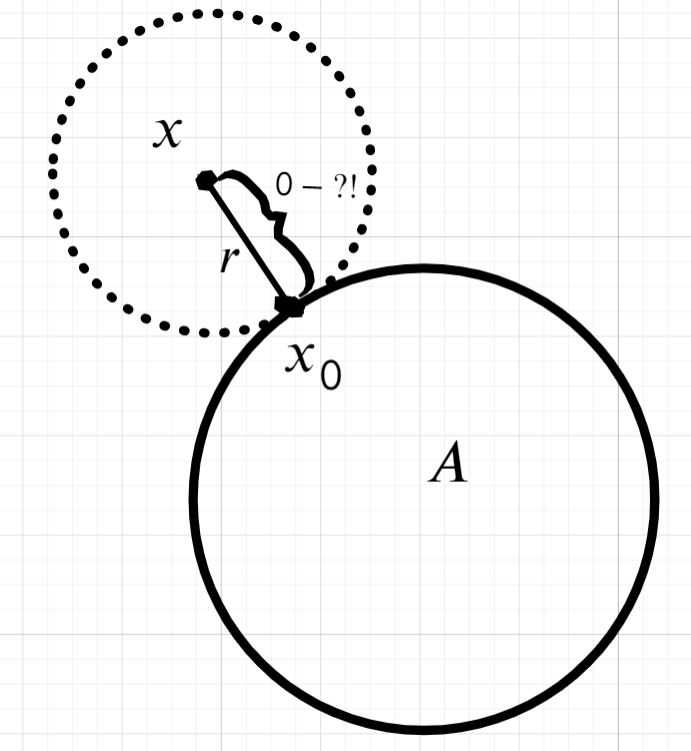
\includegraphics[scale=0.4]{01.png}$$
		$\Leftarrow)$ $x \in A \Rightarrow \rho(x, A) = \underset{x_0 \in A}{\inf}\Norm{x -x_0} = \Norm{x - x} = 0.$ 
		\end{Proof}
		\item Доказать, что для того, чтобы элемент $x \in H$ был ортогонален подпространству $L \subset H$ необходимо и достаточно, чтобы для любого элемента $y \in L$ имело место неравенство $\|x\| \leqslant\|x-y\|$.
		\begin{Proof}
			$x \in H$, $L\subset H$. $$x\perp L \Longleftrightarrow \forall y \in L \quad \Norm{x} \leq \Norm{x-y}.$$
		\begin{multline*}
			\Norm{x-y} = \sqrt{(x-y, x-y)} = \sqrt{(x,x) - (y,x) - (x,y) + (y,y)} =\\= [x\perp L \Longleftrightarrow (x,y) = 0\forall y \in L] = \sqrt{(x,x) + (y,y)}\leq \sqrt{(x,x)} + \sqrt{(y,y)} = \Norm{x} + \Norm{y}.
		\end{multline*}
		\end{Proof}
		\item Доказать, что для любого множества $M \subset H$ множество $M^{\perp} \subset H$ является подпространством в $H$.
		\begin{Proof}
			Доказательство проведем аналогично теореме о том, что ортогональное дополнение является подпространством. Имеем $M \subset H$. Тогда \begin{enumerate}
			\item $M^\perp$ --- линейное многообразие, т.е. $$\forall z_1, z_2 \in M^\perp, \alpha,\beta \quad (\alpha z_1 + \beta z_2, m) = \alpha(z_1,m) + \beta(z_2,m) = 0\ \forall m \in M$$
			Это значит, что $(\alpha z_1 +\beta z_2) \in M^\perp$.
			\item $M^\perp$ --- замкнутое множество (предел любой последовательности из $M^\perp$ лежит внутри $M^\perp$). Действительно $$\forall (z_n)\in M^\perp: z_n \xrightarrow[n\to\infty]{H}z, \quad \forall m \in M\ (z_n, m) = 0 \xrightarrow[n\to\infty]{} (z, m) =0\Rightarrow z \in M\perp.$$
		\end{enumerate}
		\end{Proof}
		\item Пусть $A, B \subset E$ и $\bar{A} \subset \bar{B}$. Следует ли, что $A \subset B$. Ответ обоснуйте и приведите пример.
		 \begin{Proof}
		 	Не следует. Данное свойство будет выполняться в том случае, когда оба множества являются замкнутыми. Однако, если они не замкнуты, то это неверно. Например, если $$A = \{0\} \cup \Big\{\dfrac{1}{n}\Big\}_{n=1}^{\infty},\quad B = \Big\{\dfrac{1}{n}\Big\}_{n=1}^{\infty}.$$ Во множестве $A$ точка 0 не изолированная и не предельная, а остальные --- изолированные. Следовательно, они образуют замыкание $\overline{A}$. В $B$ все точки изолированные, следовательно, они также образуют замыкание $\overline{B}$. Однако $A \not \subset B$.
		 \end{Proof}
		\item Доказать, что пространство $\ell_{2}$ является строго нормированным.
		\begin{Proof}
			Для доказательства того, что $l_2$ строго нормированное, рассмотрим условие строгой нормированности: $$\Norm{x + y} = \Norm{x} + \Norm{y}$$
		В $l_2$
		$$\sqrt{\sum_{i=1}^{\infty}(x_i + y_i)^2} = \sqrt{\sum_{i=1}^{\infty}(x_i)^2}+ \sqrt{\sum_{i=1}^{\infty}(y_i)^2}$$
		Возведем обе части в квадрат
		$$\sum_{i=1}^{\infty}(x_i + y_i)^2 =\sum_{i=1}^{\infty}(x_i)^2 + 2\sqrt{\sum_{i=1}^{\infty}(x_i)^2} \sqrt{\sum_{i=1}^{\infty}(y_i)^2} + \sum_{i=1}^{\infty}(y_i)^2$$
		Раскроем левое выражение
		$$\sum_{i=1}^{\infty}x_i^2 + \sum_{i=1}^{\infty}y_i^2 + 2\sum_{i=1}^{\infty}x_iy_i =\sum_{i=1}^{\infty}x_i^2 + 2\sqrt{\sum_{i=1}^{\infty}x_i^2} \sqrt{\sum_{i=1}^{\infty}y_i^2} + \sum_{i=1}^{\infty}y_i^2$$
		$$\sum_{i=1}^{\infty}x_iy_i = \sqrt{\sum_{i=1}^{\infty}x_i^2} \sqrt{\sum_{i=1}^{\infty}y_i^2}$$
		Заметим, что это эквивалентно $$(x,y) = \Norm{x}\Norm{y}.$$
		С учетом того, что $(x,y)^2 = (x,y)(x,y) = [y=\lambda x] = (x,x)(y,y) = \Norm{x}^2\Norm{y}^2$.\\\\
		То есть, это равенство верно тогда и только тогда, когда $y = \lambda x$.
		\end{Proof}
		\item  Доказать, что любое гильбертово пространство является строго нормированным.
		\begin{Proof}
			Покажем, что произвольное $H$ строго нормированное, то есть $$\Norm{x+y} = \Norm{x} + \Norm{y}\Longleftrightarrow y = \lambda x,\ \lambda > 0$$
		\begin{multline*}
			\Norm{x+y}^2 = (x+y,x+y) = (x,x) + (x,y) + (y,x) + (y,y) = \Norm{x}^2 + \Norm{y}^2 + 2(x,y) =\\= \begin{bmatrix}
				(x,y)^2 = (x,y)(x,y) = [y=\lambda x] =\\= (x,x)(y,y) = \Norm{x}^2\Norm{y}^2
			\end{bmatrix} = \Norm{x}^2 + \Norm{y}^2 + 2\Norm{x}\Norm{y} = \Big(\Norm{x} + \Norm{y}\Big)^2.
		\end{multline*}
		\end{Proof}
		\item Доказать, что ортогональная система без нулевого элемента линейно независима в гильбертовом пространстве.
		\begin{Proof}
			Возьмем систему $\{\varphi_j\}_{j=1}^{\infty}, \varphi_j \ne 0\ \forall j.$
		Система ортогональная, то есть $$(\varphi_i, \varphi_j) = 0,\ i\ne j.$$
		Возьмем произвольную конечную подсистему и рассмотрим линейную комбинацию $$\alpha_1 \varphi_1 + \ldots + \alpha_n \varphi_n = 0.$$
		Домножаем скалярно на $\varphi_k$, $k=\overline{1,n}$. Тогда $$\alpha_k\underset{\ne 0}{(\varphi_k,\varphi_k)} = 0 \Rightarrow \alpha_k = 0,\ k =\overline{1,n}.$$
		То есть любая конечная подсистема линейно независимая $\Rightarrow$ исходная система линейно независимая.
		\end{Proof}
		\item Доказать, что для любого множества $M \subset H$ в гильбертовом пространстве $H$ имеет место включение $M \subset\left(M^{\perp}\right)^{\perp}$. Привести пример строгого включения.
		\begin{Proof}
			Возьмем произвольный $x \in M$. Он ортогонален всем $y \in M^\perp$. Если теперь взять произвольный $y \in M^\perp$, то он будет ортогонален всем $x \in (M^\perp)^\perp$. Таким образом, $M \subseteq (M^\perp)^\perp$.\\\\
		Приведем пример строго включения. Рассмотрим $$M = \{x \in l_2 : x = (x_1,\ldots, x_n, 0,\ldots)\}$$
		Для него $$M^\perp = \{z \in l_2 : z = (z_1,\ldots, z_n, z_{n+1},\ldots),\ (z,x) = 0\ \forall x \in M\}$$
		А для него $$(M^\perp)^\perp = \{x \in l_2 : x = (x_1,\ldots, x_n, x_{n+1},\ldots),\ (x,z) = 0\ \forall z \in M^\perp\}$$
		Таким образом, $M \subset (M^\perp)^\perp$.
		\end{Proof}
		\item Пусть $M \subset E$ выпуклое множество и $\alpha$ - некоторое число. Доказать, что множество $\alpha M=\{x \in E \mid x=\alpha y, y \in M\}$ - выпукло. Будет ли множество всех выпуклых подмножеств пространства $E$ векторным пространством?
		\begin{Proof}
			Пусть $M\subset E$ --- выпуклое множество и $\alpha$ --- некоторое число. Доказать, что множество $\alpha M = \{x \in E | x = \alpha y, y \in M\}$ выпукло. Будет ли множество всех выпуклых подмножеств пространства $E$ векторным пространством?\\\\
		Возьмем $x_1, x_2 \in \alpha M$. Тогда $\exists y_1, y_2 \in M : x_1 = \alpha y_1,\ x_2 = \alpha y_2$.
		Нам известно, что $$\lambda y_1 + (1-\lambda)y_2 \in M,$$ т.е. $M$ --- выпуклое. Проверим для $\alpha M$ $$\lambda x_1 + (1-\lambda)x_2 = \lambda(\alpha y_1) + (1-\lambda)(\alpha y_2) = \alpha( \lambda y_1 + (1-\lambda)y_2)\in \alpha M.$$
		Что означает выпуклость $\alpha M$.\\\\
		Для второго пункта приведем пример. Рассмотрим $E = \Rm^2$ и на нем множества $$A = \{(x,0) | x \in \Rm\},\quad B = \{(0,y) | y \in \Rm\}.$$
		Они выпуклы. Но если взять $C = A \cup B$, то оно уже не будет выпуклым, т.к. мы не сможем провести отрезок между $(0,1)$ и $(1,0)$ $$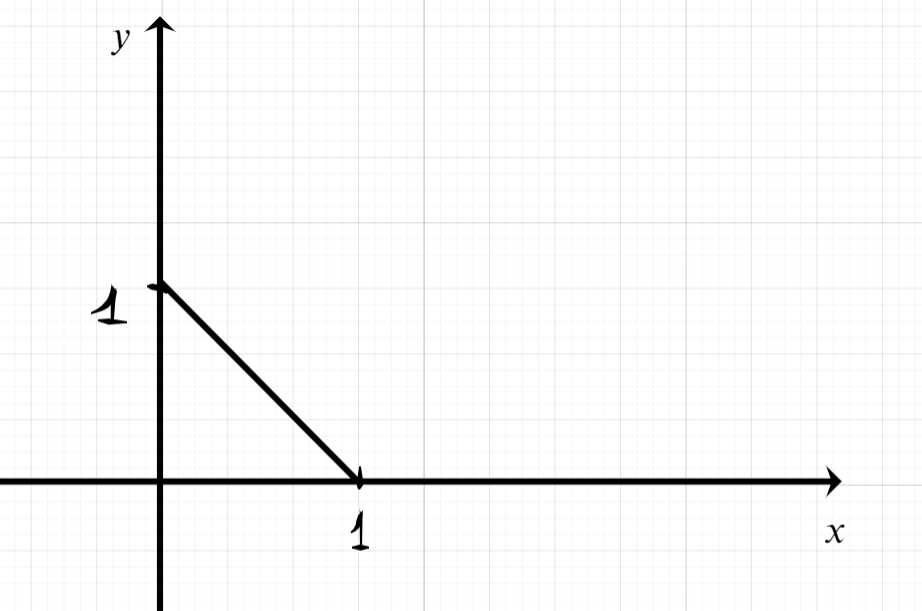
\includegraphics[scale=0.4]{02.png}$$
		\end{Proof}
		\item Будет ли замыкание выпуклого множества $M \subset E$ в нормированном векторном пространстве $E$ выпуклым множеством? Ответ обоснуйте.
		\begin{Proof}
			Рассмотрим замыкание $\overline{M}$ множества $M \subset E$. Замыкание множества представляет собой объединение внутренних и предельных точек множества. Пусть $x, y\in \overline{M}$ --- предельные точки $M$ (иначе очевидно выполняется). Тогда в $M$ найдутся последовательности, которые сходятся к этим точкам. Пусть это $x_n$ и $y_n$. Очевидно, что раз все точки этих последовательностей лежат в $M$, то $$\lambda x_n + (1-\lambda)y_n \in M.$$
		При стремлении $n\to \infty$ получим $$\lambda x_n + (1-\lambda)y_n \to \lambda x + (1-\lambda)y \in \overline{M}.$$
		Значит $\overline{M}$ выпукло.
		\end{Proof}
		\item Пусть $A, B \subset E$ - замкнутые множества и их пересечение $A \cap B$ пусто. Может ли расстояние $\rho(A, B)=0$ ?
		\begin{Proof}
			От противного. Пусть $A, B \subset E$ --- замкнутые множества и $A \cap B = \varnothing$, причем $\rho(A,B) = 0$. Поскольку $\rho(A,B) = \rho(a, b) = 0$, $a\in A$, $b \in B$, то $a = b$. Но $A \cap B = \varnothing$. Получили противоречие.
		\end{Proof}
		\item Пусть $M$ и $N$ - подпространства гильбертова пространства $H$ и $M \perp N$. Доказать, что $M$ и $N$ - подпространство в $H$.\\\\
		
		\item Пусть $M, N \subset H$ и $H=M+N$ Верно ли, что $N=M^{\perp}$.\\\\
		
		\item Пусть $M, N \subset H$ такие, что любой $x \in H$ единственным образом представим в виде $x=y+z, y \in N, z \in M$. Следует ли отсюда, что $N$ и $M$ - подпространства в $H$. Ответ обосновать.\\\\
		
		\item  Доказать, что в пространстве со скалярным произведением выполнено равенство$$
		\|z-x\|^{2}+\|z-y\|^{2}=\frac{1}{2}\|x-y\|^{2}+2\left\|z-\frac{x+y}{2}\right\|^{2} .
		$$
		\begin{Proof}
			В пространстве введено скалярное произведение $\Rightarrow$ можно воспользоваться равенством параллелограмма \begin{multline*}
			\Norm{z - x}^2 + \Norm{z - y}^2 = \dfrac{1}{2}\Big(\Norm{z - y - (z - x)}^2 + \Norm{z - x + z - y}^2\Big) =\\= \dfrac{1}{2}\Norm{x-y} + \dfrac{1}{2}\Norm{2 z - (x+y)} = \dfrac{1}{2}\Norm{x-y} + 2\Norm{z - \dfrac{x+y}{2}}
		\end{multline*}
		\end{Proof}
		\item Доказать, что в унитарном пространстве $H$ элементы $x$ и $y$ ортогональны тогда и только тогда, когда $$
		\|\alpha x+\beta y\|^{2}=\|\alpha x\|^{2}+\|\beta y\|^{2}, \quad \forall \alpha, \beta \in \mathbb{C}
		$$ 
		\begin{Proof}
			Для доказательства воспользуемся аксимомами скалярного произведения:
		\begin{multline*}
			\Norm{\alpha x + \beta y}^2 = (\alpha x + \beta y, \alpha x + \beta y) =(\alpha x, \alpha x) + (\alpha x, \beta y) + (\beta y, \alpha x) + (\beta y, \beta y) =\\= \alpha \overline{\alpha} (x,x) + \alpha \overline{\beta} (x,y) + \beta \overline{\alpha}(y,x) + \beta\overline{\beta}(y,y) = |\alpha|^2 \Norm{x}^2 + |\beta|^2 \Norm{y}^2 + \alpha \overline{\beta} (x,y) + \beta \overline{\alpha}(y,x) =\\= \Norm{\alpha x}^2 + \Norm{\beta y}^2 + \alpha \overline{\beta} (x,y) + \beta \overline{\alpha}(y,x). 
		\end{multline*}
		Для того, чтобы нужное нам равенство выполнялось, необходимо, чтобы $$\alpha \overline{\beta} (x,y) + \beta \overline{\alpha}(y,x) = 0.$$ Если $\alpha,\beta \ne 0$, то это возможно лишь при условии $$(x,y) = (y,x) = 0 \Longleftrightarrow x \perp y.$$
		\end{Proof}
		\item Доказать, что в пространстве $C[a, b]$ нельзя ввести скалярное произведение, согласованное с нормой этого пространства. \begin{Proof}
			Зададим скалярное произведение в $C[a,b]$ согласованное с нормой как $$(x,y) = \underset{t \in [a,b]}{\max}|x(t) y(t)|.$$
		Проверим, выполняются ли аксиомы скалярного произведения:\begin{enumerate}
			\item $(x,x) \geq 0$, $(x,x) = 0\Longleftrightarrow x=0$ очевидно выполняется.
			\item $(\alpha x,y) = \alpha(x,y)$.
			$$\underset{t \in [a,b]}{\max}|\alpha x(t) {y(t)}| = |\alpha|\underset{t \in [a,b]}{\max}|x(t) {y(t)}|,$$
			таким образом, эта аксиома, вообще говоря, не выполняется.
		\end{enumerate}
		\end{Proof}
		\item Пусть $\left(x^{(n)}\right)_{n=1}^{\infty},\left(y^{(n)}\right)_{n=1}^{\infty} \subset E$ - фундаментальные последовательности. Доказать, что числовая последовательность $\left.\left.\lambda_{n}=\| x^{(n)}\right)-y^{(n)}\right) \|$ сходится.
		\begin{Proof}
			$(x_n), (y_n) \subset E$ --- последовательности Коши $\Rightarrow$ каждая из них имеет предел $$x = \lim\limits_{n\to \infty}x_n,\quad y = \lim\limits_{n\to \infty}y_n.$$
		Тогда распишем $$\lambda_n = \Norm{x_n - y_n} = \Norm{x_n - x + x - y + y - y_n} \leq \Norm{x_n - x} + \Norm{x-y} + \Norm{y -y_n} \xrightarrow[n\to\infty]{} \Norm{x - y}.$$
		\end{Proof}
		\item Доказать, что если отображение $f: X \rightarrow Y$ непрерывно, то для любого $A \subset X$ справедливо включение $f(\bar{A}) \subset \overline{f(A)}$.
		\item Пусть множество $A \subset E$ фиксировано. Доказать, что функция $f(x)=$ $=\rho(x, A)$ непрерывно отображает $E$ в $\mathbb{R}$. \begin{Proof}
			Докажем, что отображение является Липшицевым, а следовательно и равномерно непрерывным. Для этого мы воспользуемся свойством инфимума и неравенством треугольника.
		\begin{multline*}
			|f(x) - f(y)| =|\rho(x,A) - \rho (y,A)|= \Big|\inf_{a \in A}\Norm{x-a} - \inf_{a \in A}\Norm{y-a}\Big|\leq\\\leq \Big|\Norm{x-a} - \Norm{y-a}\Big|\leq \Norm{x - a - (y-a)} = \Norm{x-y}.
		\end{multline*}
		То есть отображение Липшицево, значит непрерывно.
		\end{Proof}
		\item Образует ли в пространстве $C[0,1]$ подпространство множество многочленов степени не выше чем $n$ ?
		\begin{Proof}
			Обозначим это множество как $$P = \{a_0 + a_1x + \ldots + a_nx^n | a_i \in \Rm\}.$$
		Чтобы оно являлось подпространством, необходимо, чтобы оно было замкнуто относительно тех же операций, что и $C[0,1]$. Проверим это:\begin{enumerate}
			\item $\forall f(x), g(x) \in P$ $f(x) + g(x) \in P$.
			\item $\forall f(x) \in P, \alpha \in \Rm$ $\alpha f(x) \in P$
		\end{enumerate}
		При выполнении этих операций мы не выходим за границы множества $P$, следовательно, обе операции выполняются и $P$ является подпространством $C[0,1]$.
		\end{Proof}
		\item Функция $f$ определена и непрерывна на всей числовой прямой. Доказать, что множество $\{t \in \mathbb{R}: f(t)<1\}$ открыто на числовой прямой.
		\begin{Proof}
			Необходимо доказать, что $A = \{t \in \Rm | f(t) < 1\}$ открыто при условии, что $f$ непрерывное. По определению открытого множества из того, что $\forall t_0 \in A$ $\exists \delta > 0: B(x, \delta)\subset A$ следует, что $\forall t \in B(t_0, \delta) \Rightarrow t \in A$. То есть, нужно показать, что если $t \in B(t_0, \delta)$, а это значит $\Norm{t -t_0} < \delta$, то $t \in A$, что означает $f(t) < 1$. Воспользуемся условием непрерывности $$\forall \epsilon > 0 \exists \delta > 0 : \forall t: {\Norm{t -t_0}< \delta} \Rightarrow \Norm{f(t)-f(t_0)}< \epsilon.$$
		$t \in B(t_0,\delta)$, значит $\lim\limits_{t\to t_0} f(t) = f(t_0) < 1$, т.к. $t_0 \in A$. Значит и $f(t) < 1$, то есть $t \in A$.
		\end{Proof}
		\item Пусть $f: X \rightarrow Y$ непрерывное отображение пространства $X$ на все пространство $Y, A$ - всюду плотное в $X$ множество. Доказать, что $f(A)-$ множество, всюду плотное в $Y$.
		
		\item Доказать, что множество $A \subset E$ является ограниченным тогда и только тогда, когда для любой последовательности $x^{(n)} \in A$ и любой последовательности $\alpha_{n} \in \mathbb{C}, \alpha_{n} \rightarrow 0$ при $n \rightarrow \infty$ последовательность $\alpha_{n} x^{(n)} \rightarrow 0$ при $n \rightarrow \infty$.
		\begin{Proof}
			$\Rightarrow)$ $A$ ограничено, т.е. $\forall x \in A$ $\exists M: \Norm{x}\leq M$
			$$\Norm{\alpha_n x^{(n)}} = |\alpha_n| \Norm{x^{(n)}}\leq |\alpha_n|M \xrightarrow[n\to\infty]{}0.$$
			$\Leftarrow)$ Возьмем $\alpha_n = 1$. Тогда если $\alpha_n x^{(n)}\to 0$, то $x^{(n)}\to 0$, т.е. множество ограничено.
		\end{Proof}
		\item Пусть $M, N \subset H$ - подпространства гильбертова пространства $H$ и $M \perp N$. Доказать, что $M+N$ - подпространство в $H$.
		\begin{Proof}
			Из условия следует, что мы можем представлять элементы $x \in M + N$ единственным образом как $x = m +n, m \in M, n \in N$.
			Исследуем замкнутость относительно сложения и относительно умножения на скаляр:
			\begin{enumerate}
				\item $\forall m_1, m_2\in M,\ n_1, n_2 \in N$ $(m_1 + n_1) + (m_2+n_2) = \underbrace{(m_1 + m_2)}_{\in M} + \underbrace{(n_1 + n_2)}_{\in N} \in M+N$ 
				\item $\forall m\in M,\ n \in N$, $\forall \alpha \in \Cm$ $\alpha(m+n) = \underbrace{\alpha m}_{\in M} + \underbrace{\alpha n}_{\in N}\in M+N$
			\end{enumerate}
			Значит $M+N$ удовлетворяет свойствам подпространства.
		\end{Proof}
		\item Пусть $E=E_{1} \times E_{2}$, где $\left(E_{1},\|\cdot\|_{1}\right),\left(E_{2},\|\cdot\|_{2}\right)$ - нормированные векторные пространства. Будет ли $E$ нормированным пространством относительно нормы
		$$
		\left\|\left(x_{1}, x_{2}\right)\right\|=\left\|x_{1}\right\|_{1}+\left\|x_{2}\right\|_{2}
		$$
		\begin{Proof}
			Проверим выполнение аксиом нормы:
			\begin{enumerate}
				\item Очевидно из свойств норм.
				\item $\Norm{\alpha(x_1,x_2)} = \Norm{(\alpha x_1, \alpha x_2)} = \Norm{\alpha x_1}_1 + \Norm{\alpha x_2}_2 = |\alpha|(\Norm{x_1}_1 + \Norm{x_2}_2)$
				\item $\Norm{(x_1, x_2) + (y_1,y_2)} = \Norm{(x_1+y_1, x_2 + y_2)} = \Norm{x_1+y_1}_1 + \Norm{x_2 + y_2}_2 \leq \Norm{x_1}_1 + \Norm{y_1}_1 + \Norm{x_2}_2 + \Norm{y_2}_2 = \Norm{(x_1, x_2)} + \Norm{(y_1,y_2)}$
			\end{enumerate}
		\end{Proof}
		\item В пространстве $m$ ограниченных числовых последовательностей с нормой $\|x\|=\sup _{i}\left|x_{i}\right|$ построить замыкание множества
		$$
		A=\left\{x\left(x_{1}, \ldots, x_{i}, \ldots\right): \sum_{i=1}^{n}\left|x_{i}\right|<\infty\right\}
		$$
		\item Пусть $A, B \subset E$ - всюду плотные множества в нормированном пространстве $E$. Возможно ли, что $A \cap B=\varnothing$ ?
		\begin{Proof}
			Если рассмотреть всюду плотные множества $\mathbb{Q}$ и $\Rm\backslash \mathbb{Q}$ в пространстве $\Rm$. Их пересечение $\mathbb{Q}\cap \Rm\backslash \mathbb{Q} = \varnothing$
		\end{Proof}
		\item Пусть $E$ - вещественное нормированное пространство, $x, y \in E$. Доказать, что функция $f(t)=\|x-t y\|, t \in \mathbb{R}$, достигает своей точной нижней грани.
		\item В пространстве непрерывно дифференцируемых на отрезке $[a, b]$ функций $C^{(1)}[a, b]$ введем норму по формуле
		$$
		\|x\|=\left(\int_{a}^{b}\left(|x(t)|^{2}+\left|x^{\prime}(t)\right|^{2}\right) \mathrm{d} t\right)^{1 / 2}
		$$
		Будет ли пространство $C^{1}[a, b]$ банаховым?
		\begin{Proof}
			Возьмем отрезок $[0,1]$ и на нем последовательность Коши $x_n(t) = \sin(\pi n t)$. Она сходится поточечно к $x = 0$. Но $x_n'(t) = \pi n \cos (\pi n t)$ не сходится на отрезке. Таким образом, последовательность Коши не сходится по норме, а значит это пространство не является банаховым.
		\end{Proof}
		\item Пусть $A, B \subset E-$ произвольные множества в нормированном пространстве $E$, причем $\rho_{x}(A, B)=0$. Возможно ли, что $\rho_{y}(f(A), f(b)) \neq 0$, если $f: X \rightarrow Y$ есть:
		\begin{itemize}
		\item непрерывное отображение;
		
		\item равномерно непрерывное отображение?
		
		\end{itemize}
		\item Доказать, что непрерывное отображение $f: \mathbb{R} \rightarrow \mathbb{R}$, обладающее тем свойством, что образ каждого открытого множества есть открытое множество, - монотонная функция.
		
		\item Привести пример последовательности непустых замкнутых множеств $E_{n}$ в банаховом пространстве $E$ таких, что
		\begin{enumerate}
		\item $E_{n+1} \subset E_{n}, n=1,2, \ldots$;
		\item $\bigcap_{n=1}^{\infty} F_{n}$ пусто.
		\end{enumerate}
		\begin{Proof}
			Возьмем пространство $E = m$. В нем зададим $$E_n = \{x \in m | x =(x_1,\ldots, x_n, 0,\ldots)\}$$
			Тогда  $$E_{n+1} = \{x \in m | x =(x_1,\ldots, x_n, x_{n+1},0,\ldots)\}$$
			Тогда $E_{n+1} \subset E_n$. $\bigcap_{n=1}^\infty E_n = \varnothing$, т.к. присутствует последовательность вида $x=(1, \dfrac{1}{2},\ldots, \dfrac{1}{k},\ldots)$, у которой бесконечное число ненулевых элементов. Она не принадлежит ни одному $E_n$. 
		\end{Proof}
		\item Между реками (непрерывными кривыми на плоскости, содержащими концы) $\Gamma_{1}$ и $\Gamma_{2}$, нужно построить канал (отрезок). Предположим, что расстояние между реками - длина самого короткого из возможных каналов, т. е.
		$$
		\rho\left(\Gamma_{1}, \Gamma_{2}\right)=\min _{x \in \Gamma_{1}, y \in \Gamma_{2}}\|x-y\| .
		$$
		Задает ли данная функция метрику на множестве всех рек?
		\item Рассмотрим множество $C_{\alpha}[a, b], \alpha \in(0,1]$, всех непрерывных на $[a, b]$ функций, для которых выполняется условие Гельдера
		$$
		K_{\alpha}(x)=\sup _{t_{1}, t_{2} \in[a, b], t_{1} \neq t_{2}} \frac{\left|x\left(t_{1}\right)-x\left(t_{2}\right)\right|}{\left|t_{1}-t_{2}\right|^{\alpha}}<+\infty
		$$
		Покажите, что $C_{\alpha}[a, b]$ будет нормированным пространством, если в нем норму задать как
		$$
		\|x\|_{\alpha}=\|x\|_{C[a, b]}+K_{\alpha}(x) .
		$$
		\begin{Proof}
			Проверим выполнение аксиом нормы:
			\begin{enumerate}
				\item $\Norm{x}_\alpha \geq 0$ (т.к. оба слагаемых неотрицательны) и $\Norm{x}_\alpha = 0 \Longleftrightarrow x(t) = 0$ на $[a,b]$.
				\item $\Norm{a x}_\alpha = \max|a x(t)| + \sup _{t_{1}, t_{2} \in[a, b], t_{1} \neq t_{2}} \frac{\left|ax\left(t_{1}\right)-ax\left(t_{2}\right)\right|}{\left|t_{1}-t_{2}\right|^{\alpha}} =\\= |a| \max|x(t)| + |a| \sup _{t_{1}, t_{2} \in[a, b], t_{1} \neq t_{2}} \frac{\left|x\left(t_{1}\right)-x\left(t_{2}\right)\right|}{\left|t_{1}-t_{2}\right|^{\alpha}} = |a| \Norm{x}_\alpha$
				\item $\Norm{x + y}_\alpha = \max|x(t) + y(t)| + \sup _{t_{1}, t_{2} \in[a, b], t_{1} \neq t_{2}} \frac{\left|x\left(t_{1}\right)-x\left(t_{2}\right) + y(t_1)-y(t_2)\right|}{\left|t_{1}-t_{2}\right|^{\alpha}} \leq \max|x(t)| + \max|y(t)| + \sup _{t_{1}, t_{2} \in[a, b], t_{1} \neq t_{2}} \frac{\left|x\left(t_{1}\right)-x\left(t_{2}\right)\right|}{\left|t_{1}-t_{2}\right|^{\alpha}} + \sup _{t_{1}, t_{2} \in[a, b], t_{1} \neq t_{2}} \frac{\left|y\left(t_{1}\right)-y\left(t_{2}\right)\right|}{\left|t_{1}-t_{2}\right|^{\alpha}} = \Norm{x}_\alpha + \Norm{y}_\alpha$
 			\end{enumerate}
 			Все свойства выполнены, значит это пространство будет нормированным.
		\end{Proof}
	
			\end{enumerate}
\end{document}